\documentclass[aspectratio=169]{beamer}

% Use T1 font encoding for better font output
\usepackage[T1]{fontenc}
\usepackage[utf8]{inputenc}
\usepackage{graphicx}
\graphicspath{{.}{graphics}}
\usepackage{amsmath,amssymb,mathtools}
\usepackage{sfmath}
\usepackage{helvet}
\usepackage{tikz}
% \usepackage{movie15}
\usepackage{animate}
\usepackage{hyperref}
\usepackage{physics}
\usepackage{xcolor}
\usepackage[absolute,overlay]{textpos}
\usepackage{xparse}
\renewcommand{\rmdefault}{cmss}
\renewcommand{\sfdefault}{cmss}

%%%%%%%%%%%%% Maths Abbrevs %%%%%%%%%%%%%
\newcommand{\iu}{\ensuremath{\mathrm{i}}}
\newcommand{\kB}{\ensuremath{k_\mathrm{B}}}
\NewDocumentCommand{\eu}{ !o }{ 
	% function associated with a symmetry operation and bead number
	\IfNoValueTF{#1}
		{\ensuremath{\mathrm{e}}}
		{\ensuremath{\mathrm{e}^{#1}}}
}




% % Set sans-serif as the default font family
% \renewcommand{\familydefault}{\sfdefault}

% Define custom color

\definecolor{customblue}{HTML}{3059A0}
\definecolor{slidegray}{HTML}{808080}
\definecolor{commentgray}{HTML}{666666}

% Customize title slide
\setbeamercolor{title}{fg=customblue}
\setbeamerfont{title}{series=\bfseries, size=\fontsize{14pt}{18pt}\selectfont}
\setbeamerfont{subtitle}{series=\bfseries, size=\fontsize{14pt}{18pt}\selectfont}
\setbeamercolor{author}{fg=slidegray}
\setbeamerfont{author}{size=\fontsize{12pt}{14pt}\selectfont}
\setbeamercolor{institute}{fg=slidegray}
\setbeamerfont{institute}{size=\small, size=\fontsize{10pt}{12pt}\selectfont}
\setbeamercolor{eqn head}{fg=red!50!black, bg=black!10}
\setbeamercolor{eqn}{bg=white}
% \setbeamerfont{button}{size=\fontsize{9pt}{11pt}\selectfont}
\setbeamercolor{button}{fg=red!50!black, bg=black!10}
\setbeamercolor{button border}{fg=black!50}
\setbeamercolor{alerted text}{fg=red}

\makeatletter
\setbeamertemplate{title page}{
  \vbox{}
  \begin{centering}


    % Row of logos
    
    \begin{textblock*}{\paperwidth}(0pt,30pt)
        \noindent
      \hspace*{\fill}
      
\includegraphics[height=1cm]{logos/ipi-logo.pdf} \hfill
      
\includegraphics[height=1.2cm]{logos/mpsd-mini-logo.png} \hfill
      
\includegraphics[height=1cm]{logos/minerva_logo_green.pdf} \hfill
      \includegraphics[height=1.15cm]{logos/sabia-logo.pdf} \hfill
      
\includegraphics[height=1cm]{logos/AvH_Logo_P353C.eps} \hfill
      
\includegraphics[height=1cm]{logos/marie_curie_action.JPG}
      \hspace*{\fill}
    \end{textblock*}

    \vskip6em
    %% TITLE %%
    \begin{beamercolorbox}[center]{title}
      \usebeamerfont{title}\inserttitle\par
    \end{beamercolorbox}
        \vskip0.5em
    \begin{beamercolorbox}[center]{subtitle}
      \usebeamerfont{subtitle}\insertsubtitle\par
    \end{beamercolorbox}
        \vskip1.5em
    %% AUTHORS %%
    \begin{beamercolorbox}[center]{author}
      \usebeamerfont{author}\insertauthor
    \end{beamercolorbox}
        \vskip0.5em
    %% INSTITUTE %%
    \begin{beamercolorbox}[center]{institute}
      \usebeamerfont{institute}\insertinstitute
    \end{beamercolorbox}
    \vskip1.5em
    %% DATE %%
    \begin{beamercolorbox}[center]{date}
      \usebeamerfont{date}\insertdate
    \end{beamercolorbox}
  \end{centering}
}
\makeatother


% Set frame title colors
\setbeamercolor{frametitle}{bg=customblue, fg=white}
\setbeamerfont{frametitle}{series=\bfseries\boldmath}


% Customize the frame title to have a colored band with white text
\newlength{\headerheight}
\setlength{\headerheight}{25pt}
\newlength{\headerdepth}
\setlength{\headerdepth}{15pt}
\newlength{\headertotal}
\setlength{\headertotal}{\dimexpr\headerheight+\headerdepth\relax}
\setbeamertemplate{frametitle}{
  \nointerlineskip%
  \begin{beamercolorbox}[wd=\paperwidth, ht=\the\headerheight, dp=\the\headerdepth, leftskip=1em]{frametitle}
    \usebeamerfont{frametitle}\insertframetitle
  \end{beamercolorbox}
}

% Remove navigation symbols
\setbeamertemplate{navigation symbols}{}

% Customize itemized lists
\setbeamercolor{item}{fg=customblue}
\setbeamertemplate{itemize item}{\raise0.1ex\hbox{\large$\bullet$}}




\setbeamertemplate{footline}{
  \raisebox{1em}{%
    \makebox[\paperwidth]{%
      \hfill
      \color{slidegray}\scriptsize\insertframenumber
      \hspace{1em}
    }
  }
}



% Title information
\title{Path-Integral Molecular Dynamics}
\subtitle{Turning Nuclei Quantum}
\author{George Trenins, Hannah Bertschi, Jorge Castro, and Mariana Rossi}
\institute{MPI for the Structure and Dynamics of Matter, Hamburg}
\date{2 July 2025, CNPEM/Ilum -- Max Planck Meeting}


\begin{document}

% Title page
{
  \setbeamertemplate{footline}{}
  \begin{frame}
    \titlepage
  \end{frame}
}

\section{Outline}

\begin{frame}
  \frametitle{Outline}
  \begin{center}
    \onslide<1->{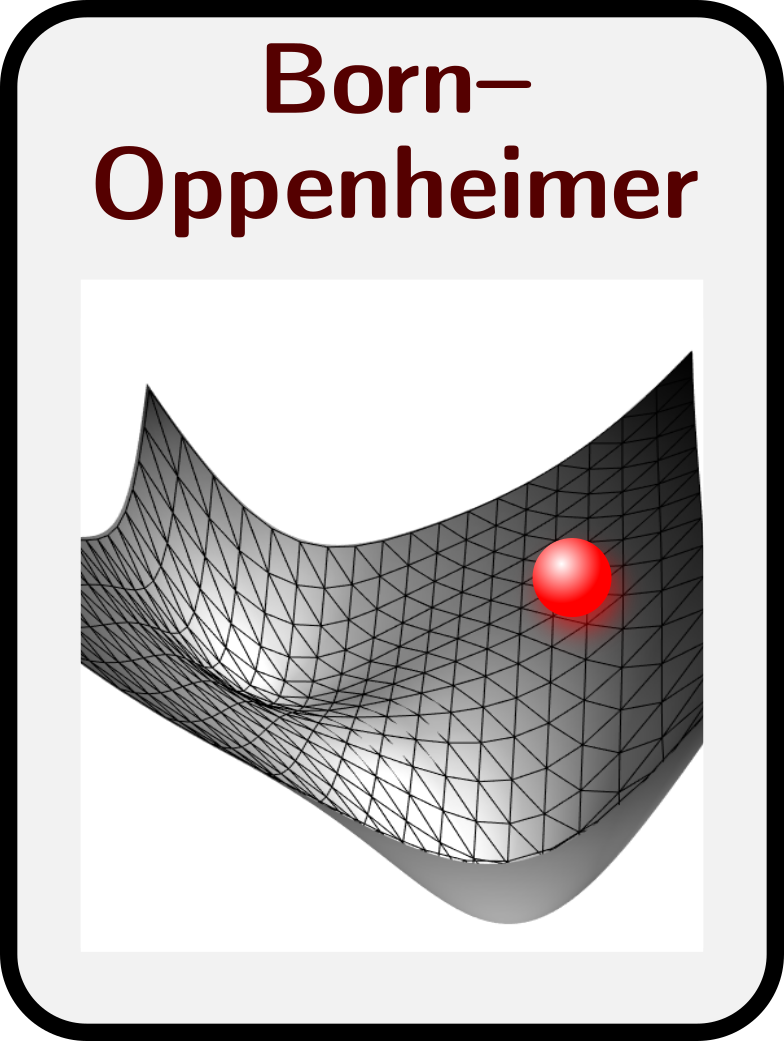
\includegraphics[width=0.23\textwidth]{outline-0.png}}
    \hfill
    \onslide<2->{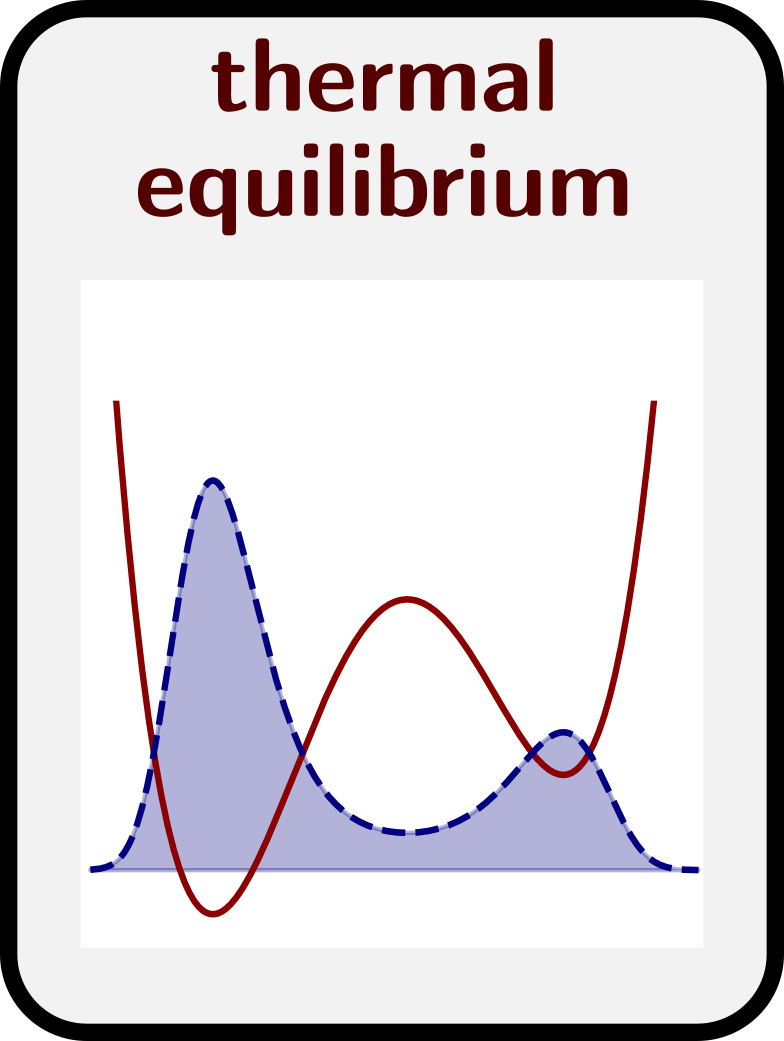
\includegraphics[width=0.23\textwidth]{outline-1.png}}
    \hfill
    \onslide<3->{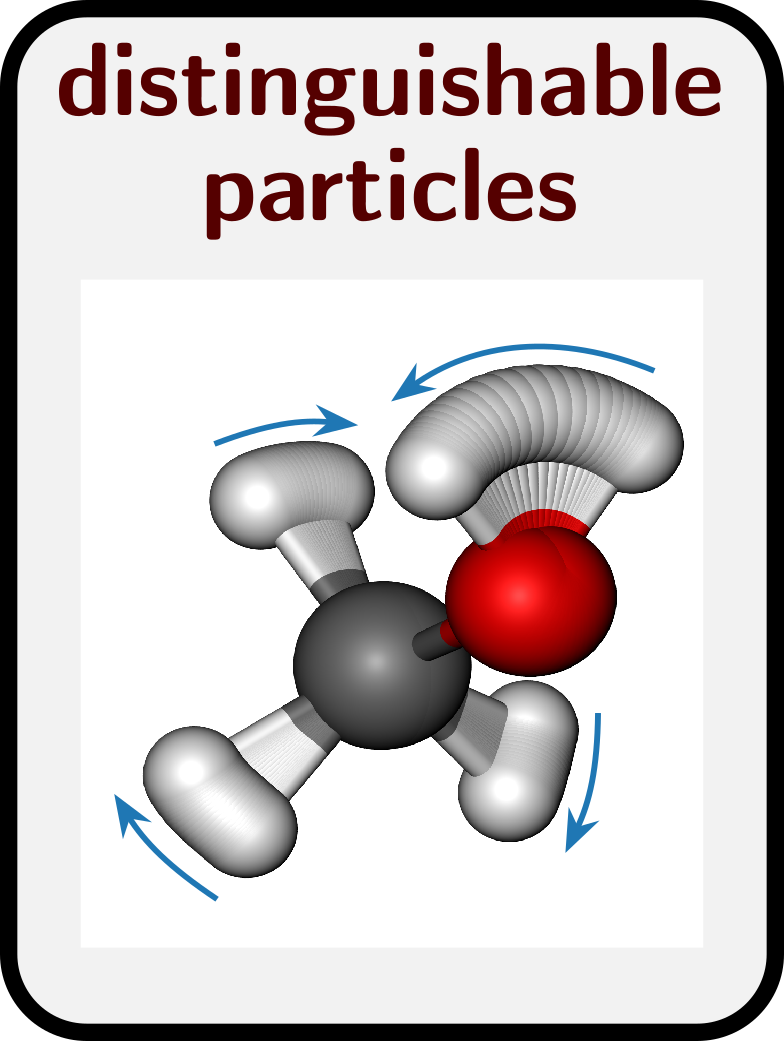
\includegraphics[width=0.23\textwidth]{outline-2.png}}
    \hfill
    \onslide<4->{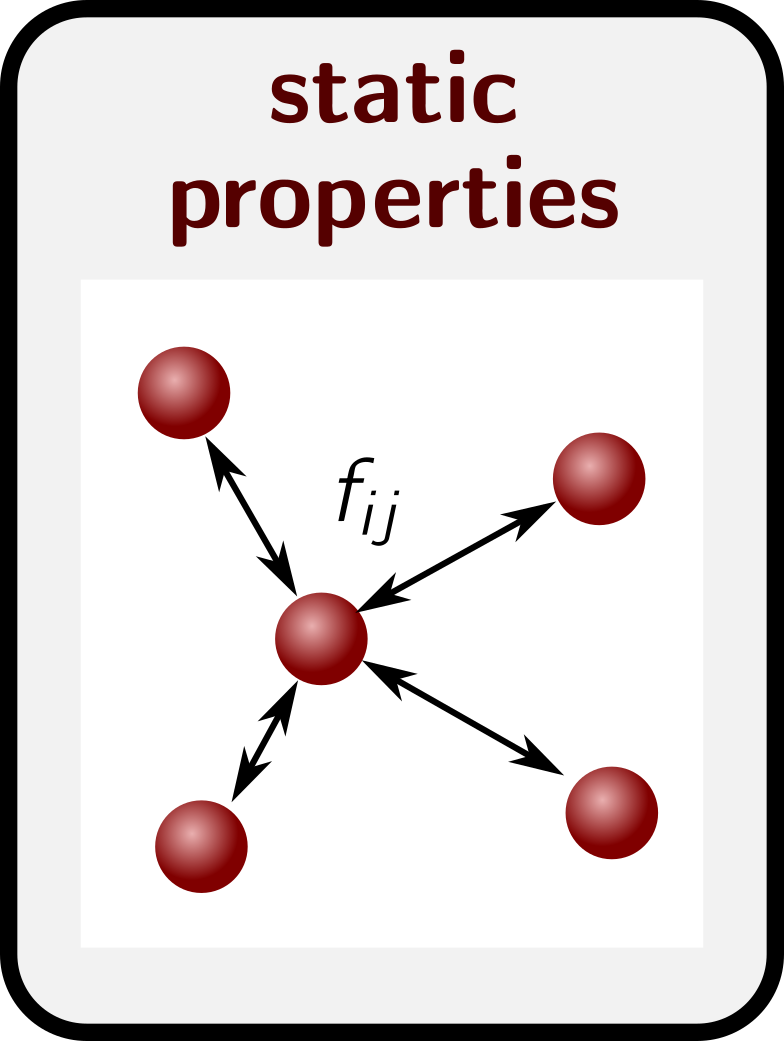
\includegraphics[width=0.23\textwidth]{outline-3.png}}
  \end{center}
\end{frame}

\section{Partition function}


\begin{frame}
    \frametitle{The partition function}

    \bigskip
  
    $\displaystyle\hspace*{3em}
    \vphantom{\sum_n}
    Z = \Tr[\eu[-\beta \hat{H}]]  
    \onslide*<5->{{} = \sum_n \! \mel{\psi_n}{ \eu[-\beta \hat{H}] }{\psi_n}}
    \onslide*<5>{
       {} = \sum_n \! \mel{\psi_n}{  \eu[-\beta E_n]  }{\psi_n} 
    }
    \onslide*<6->{
       {} = \sum_n \eu[-\beta E_n] \bra{\psi_n} \ket{\psi_n}  
    }
    \onslide*<6->{
        = \sum_n \eu[-\beta E_n]
    }
    $

    \begin{columns}[T]
        \begin{column}{0.35\textwidth}
            \onslide<3->{
            \begin{center}
                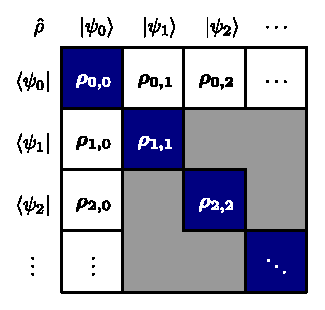
\includegraphics[scale=0.9]{trace.eps}
            \end{center}}
        \end{column}

        \begin{column}{0.6\textwidth}
            \begin{overlayarea}{\textwidth}{0.55\textheight}
                \vspace*{0.05ex}
                \onslide*<4-5>{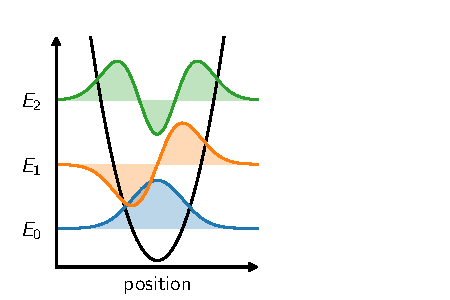
\includegraphics[width=2.9in]{qho0.pdf}}
                 \onslide*<6->{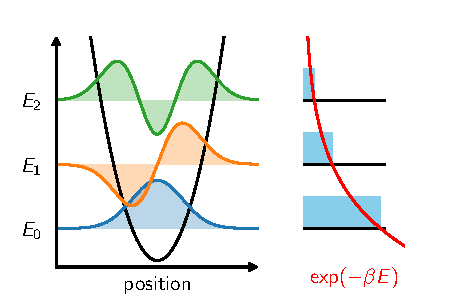
\includegraphics[width=2.9in]{qho1.pdf}}
            \end{overlayarea}
        \end{column}
        
    \end{columns}

    \begin{textblock*}{\paperwidth}(65pt,50pt)
        \noindent
        \onslide<2->{${\color{red!50!black}\beta = 1/k_{\mathsf{B}}T}$}
    \end{textblock*}
  
\end{frame}

\section{Classical limit}

\begin{frame}
    \frametitle{Splitting up}

    \bigskip

    \begin{overprint}
        $\displaystyle
        \vphantom{\int_{-\infty}^{\infty}}
        Z = \onslide*<1>{\Tr[\eu[-\beta \hat{H}]]}
            \onslide*<2->{\Tr[\eu[-\beta (\alert<2>{\hat{K} + \hat{U}})]]}
            \onslide*<4->{
                {} \sim \Tr[\eu[-\beta \hat{K}] \eu[-\beta \hat{U}]]}
            \onslide*<5-6>{
                = \int_{-\infty}^{\infty} \dd{X} \bra{X} \! \eu[-\beta \hat{K}] \alert<6>{\eu[-\beta \hat{U}]  \! \ket{X}}
            }
            \onslide*<7->{
                = \int_{-\infty}^{\infty} \dd{X} \mel{X}{ \eu[-\beta \hat{K}]}{X} \alert<7>{\eu[-\beta U(X)] }
            }
            \onslide*<4->{,
            \quad \beta \to 0
            }
        $
    \end{overprint}

    \bigskip

    \begin{overprint}
        \begin{center}
            
            \begin{minipage}{0.65\textwidth}
                \onslide<3->{
                \begin{beamerboxesrounded}[lower=eqn,upper=eqn head,shadow=true]{\bfseries%
                    Trotter formula}
                    \centering
                    $ \rule[-0.75em]{0pt}{2.5em} 
                    \eu[ -\beta (\hat{K} + \hat{U})] \sim \eu[ -\beta \hat{K}] \eu[ -\beta \hat{U}] \qty( 1 - \frac{\beta^2}{2} [ \hat{K}, \hat{U} ] ) $
                \end{beamerboxesrounded}}

                \bigskip

                \onslide<6->{
                \begin{beamerboxesrounded}[lower=eqn,upper=eqn head,shadow=true]{\bfseries%
                    Eigenvalue equation}
                    \centering
                    $ \rule[-0.75em]{0pt}{2.5em} 
                    \hat{X}\ket{X} = X \ket{X} 
                        \quad  \Rightarrow \quad 
                    \eu[-\beta U(\hat{X})] \ket{X} =  \eu[-\beta U(X)] \ket{X}
                    $
                \end{beamerboxesrounded}}
            \end{minipage}
        \end{center}
    \end{overprint}
\end{frame}

\begin{frame}
    \frametitle{Gaining momentum}

    \vspace*{2em}

    $\displaystyle
    Z \sim Z_{\text{cl}} = \int_{-\infty}^{\infty} \!\! \dd{X} 
            \onslide*<1>{\mel{X}{ \eu[-\beta \hat{K}]}{X}}
            \onslide*<2->{\mel{X}{\eu[-\beta \alert<2>{\hat{P}^2\!/2 M}]}{X}}
        \eu[-\beta U(X)] 
        \onslide*<3->{
        = \frac{1}{2\pi\hbar} \int_{-\infty}^{\infty} \!\! \dd{P} \eu[-\beta P^2\!/2 M] 
                              \int_{-\infty}^{\infty} \!\! \dd{X} \eu[-\beta U(X)]}
    $

    \smallskip


    \begin{overlayarea}{\textwidth}{0.5\textheight}
    \begin{columns}[T]
        \begin{column}{0.3\textwidth}
                \begin{center}
                    \onslide*<4>{
                        % \includemovie[
                        %     autoplay,        % start playing automatically
                        %     repeat,           % repeat video indefinitely
                        %     text={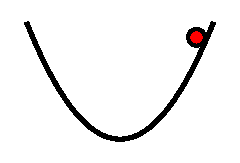
\includegraphics[page=1, width=1.75in]{clHO.pdf}}, % fallback image if poster fails
                        %     ]{1.75in}{1.185in}{graphics/clHO.mp4}%
                        \animategraphics[autoplay,loop,palindrome,width=1.75in]{18}{graphics/clHO}{}{}
                        }
                    \onslide*<5->{\includegraphics[width=1.75in, page=15]{clHO}}
                \end{center}
        \end{column}
        \begin{column}{0.6\textwidth}
            \begin{center}
                \onslide*<5->{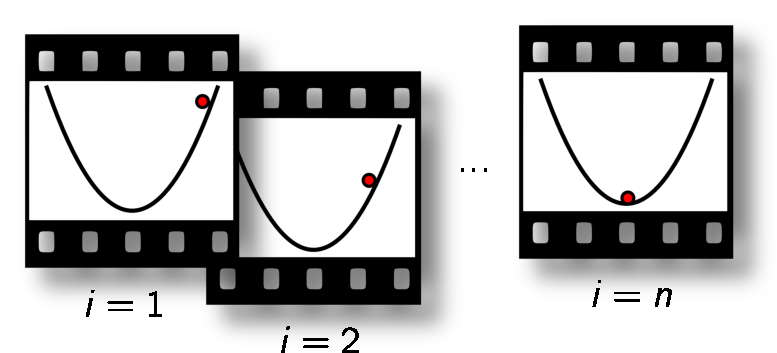
\includegraphics[scale=0.6]{clHO-frames.pdf}}
            \end{center}
        \end{column}
    \end{columns}
    \end{overlayarea}

    

\end{frame}


\section{Quantum regime}

\begin{frame}
    \frametitle{Divide and conquer}
    \begin{overlayarea}{\textwidth}{7em}
        \begin{flalign*}
            \hspace*{7em}
            Z & = \Tr[\eu[-\beta (\hat{K} + \hat{U})]]
              \sim \Tr[\eu[-\beta \hat{K}] \eu[-\beta \hat{U}]]
              \qquad (\beta \to 0)
             & \\
            \vphantom{\order{\frac{\beta^3}{N^3}}}
            \onslide+<4->{
              & = \Tr\!\Big[\qty(\eu[
                -\alert<4>{\frac{\beta}{N}} (\hat{K} + \hat{U})])^{
                    \!\!\alert<4>{N}}\Big]}
            \onslide+<5->{
                \sim \Tr\!\Big[
                        \qty(
                            \eu[-\frac{\beta}{N} \hat{K}] 
                            \eu[-\frac{\beta}{N} \hat{U}]
                            )^{\!\!N}
                    \Big] \qquad \qty(\frac{\beta}{N} \to 0) }
             &
        \end{flalign*}
    \end{overlayarea}

    \bigskip

\onslide<2->{
\begin{center}
    \begin{minipage}{0.6\textwidth}
        \begin{beamerboxesrounded}[lower=eqn,upper=eqn head,shadow=true]{\bfseries%
            Trotter formula}
            \centering
            $ \rule[-0.75em]{0pt}{2.5em} 
            \eu[ -\alert<3-4>{\epsilon} (\hat{K} + \hat{U})] \sim \eu[ -\alert<3-4>{\epsilon} \hat{K}] \eu[ -\alert<3-4>{\epsilon} \hat{U}] \qty( 1 - \alert<3-4>{\frac{\epsilon^2}{2}} [ \hat{K}, \hat{U} ] ) $
        \end{beamerboxesrounded}    
    \end{minipage}
\end{center}}
\end{frame}

\begin{frame}
    \frametitle{Identity crisis}

    \vspace*{-1em}

    \begin{overlayarea}{\textwidth}{6em}
    \begin{flalign*}
        \hspace*{3em}
          \Tr\!\Big[\qty( \eu[-\frac{\beta}{N} \hat{K}] \eu[-\frac{\beta}{N} \hat{U}] )^{\!\!N} \Big] &
        \onslide*<-3>{ {} = 
        \Tr\!\Big[\underbrace{
            \qty( \eu[-\frac{\beta}{N} \hat{K}] \eu[-\frac{\beta}{N} \hat{U}] ) \cdots 
            \qty( \eu[-\frac{\beta}{N} \hat{K}] \eu[-\frac{\beta}{N} \hat{U}] ) \cdot
            \qty( \eu[-\frac{\beta}{N} \hat{K}] \eu[-\frac{\beta}{N} \hat{U}] )}_{N\text{ times}}
         \Big] \vphantom{\qty[\prod_{l=1}^N]}} 
        \onslide*<4->{ {} = 
        \qty[ \prod_{l=1}^{N} \int \dd{X_l} 
        \mel{X_{l+1}}{ \eu[-\frac{\beta}{N} \hat{K}] }{X_l} \eu[-\frac{\beta}{N} U(X_l)] ],
        \qquad X_{N+1} \equiv X_1   }
        & 
    \end{flalign*}
\end{overlayarea}
    

    \begin{columns}[t]
        \begin{column}{0.45\textwidth}
            \onslide<2->{
            \begin{beamerboxesrounded}[lower=eqn,upper=eqn head,shadow=true]{\bfseries%
                Trace formula}
                \centering
                $ \displaystyle \Tr \hat{O} = \int_{-\infty}^{\infty} \dd{X}_l \mel{X_l}{\hat{O}}{X_l}$
            \end{beamerboxesrounded}}
        \end{column}
        \begin{column}{0.45\textwidth}
            \onslide<3->{
            \begin{beamerboxesrounded}[lower=eqn,upper=eqn head,shadow=true]{\bfseries%
                    Resolution of the identity}
                    \centering
                    $ \displaystyle \hat{I} = \int_{-\infty}^{\infty} \dd{X_l} \op{X_l}{X_l}$
            \end{beamerboxesrounded}}
        \end{column}
    \end{columns}

\end{frame}

% \begin{frame}
%     \frametitle{Identity crisis}

%     \begin{overlayarea}{\textwidth}{9em}
%     \begin{flalign*}
%         \hspace*{1.5em}
%           \Tr\!\Big[\qty( \eu[-\frac{\beta}{N} \hat{K}] \eu[-\frac{\beta}{N} \hat{U}] )^{\!\!N} \Big] &
%         \onslide*<2>{ {} = 
%         \Tr\!\Big[\underbrace{
%             \qty( \eu[-\frac{\beta}{N} \hat{K}] \eu[-\frac{\beta}{N} \hat{U}] ) \cdots 
%             \qty( \eu[-\frac{\beta}{N} \hat{K}] \eu[-\frac{\beta}{N} \hat{U}] ) \cdot
%             \qty( \eu[-\frac{\beta}{N} \hat{K}] \eu[-\frac{\beta}{N} \hat{U}] )}_{N\text{ times}}
%          \Big]} 
%         \onslide*<3->{ {} = 
%          \Tr\!\Big[\underbrace{
%             \qty( \eu[-\frac{\beta}{N} \hat{K}] \eu[-\frac{\beta}{N} \hat{U}] ) \cdot \hat{I} \cdots \hat{I} \cdot
%             \qty( \eu[-\frac{\beta}{N} \hat{K}] \eu[-\frac{\beta}{N} \hat{U}] ) \cdot \hat{I} \cdot 
%             \qty( \eu[-\frac{\beta}{N} \hat{K}] \eu[-\frac{\beta}{N} \hat{U}] )}_{N\text{ times}}
%          \Big]} &
%     \end{flalign*}
%     \onslide*<4-6>{\vspace*{-1em}
%     \[
%         \onslide*<4-5>{
%               {} = 
%         \vphantom{\qty[\prod_{l=1}^{N} \int \dd{X_l} ]}
%         \alert<4>{\int \dd{X_1}
%         \bra{X_{1}}} \!
%             \qty( \eu[-\frac{\beta}{N} \hat{K}] \eu[-\frac{\beta}{N} \hat{U}] ) \cdot \alert<5>{\hat{I}} 
%             \cdots \alert<5>{\hat{I}} \cdot
%             \qty( \eu[-\frac{\beta}{N} \hat{K}] \eu[-\frac{\beta}{N} \hat{U}] ) \cdot \alert<5>{\hat{I}} \cdot
%             \qty( \eu[-\frac{\beta}{N} \hat{K}] \eu[-\frac{\beta}{N} \hat{U}] )
%          \! \alert<4>{\ket{X_1}}  }
%         \onslide*<6>{
%           \hspace*{-2em}  {} = 
%         \qty[\alert<6>{\prod_{l=1}^{N} \int \dd{X_l}} ]
%         \bra{X_{1}}
%             \! \qty(\eu[-\frac{\beta}{N} \hat{K}] \eu[-\frac{\beta}{N} \hat{U}] )\!
%         \alert<6>{\op{X_{N}}{X_{N}}}
%             \cdots 
%         \alert<6>{\op{X_{3}}{X_{3}}}
%             \! \qty(\eu[-\frac{\beta}{N} \hat{K}] \eu[-\frac{\beta}{N} \hat{U}] )\!
%         \alert<6>{\op{X_2}{X_2}}
%             \! \qty(\eu[-\frac{\beta}{N} \hat{K}] \eu[-\frac{\beta}{N} \hat{U}] )\!
%         \ket{X_1}  } \]}
%     \onslide*<7->{\vspace*{-2em}
%     \begin{flalign*}
%         \hspace*{8em}
%         \onslide*<7>{
%           {} & = 
%         \qty[ \prod_{l=1}^{N} \int \dd{X_l} 
%         \mel{X_{l+1}}{ \eu[-\frac{\beta}{N} \hat{K}] \eu[-\frac{\beta}{N} \hat{U}] }{X_l}  ],
%         \qquad X_{N+1} \equiv X_1  & }
%         \onslide*<8>{
%           {} & = 
%         \qty[ \prod_{l=1}^{N} \int \dd{X_l} 
%         \mel{X_{l+1}}{ \eu[-\frac{\beta}{N} \hat{K}] }{X_l} \eu[-\frac{\beta}{N} U(X_l)] ],
%         \qquad X_{N+1} \equiv X_1  & }
%     \end{flalign*}}
    
%     \end{overlayarea}


%     \begin{columns}[t]
%         \begin{column}{0.45\textwidth}
%             \onslide<4->{
%             \begin{beamerboxesrounded}[lower=eqn,upper=eqn head,shadow=true]{\bfseries%
%                 Trace formula}
%                 \centering
%                 $ \displaystyle \Tr \hat{O} = \int_{-\infty}^{\infty} \dd{X}_l \mel{X_l}{\hat{O}}{X_l}$
%             \end{beamerboxesrounded}}
%         \end{column}
%         \begin{column}{0.45\textwidth}
%             \onslide<5->{
%             \begin{beamerboxesrounded}[lower=eqn,upper=eqn head,shadow=true]{\bfseries%
%                     Resolution of the identity}
%                     \centering
%                     $ \displaystyle \hat{I} = \int_{-\infty}^{\infty} \dd{X_l} \op{X_l}{X_l}$
%             \end{beamerboxesrounded}}
%         \end{column}
%     \end{columns}

% \end{frame}


\begin{frame}
    \frametitle{Element of surprise}
    \hypertarget<2>{ke-slide}{}

    \begin{equation*}
        Z  \sim \qty[ \prod_{l=1}^{N} \int \dd{X_l} 
        \mel{X_{l+1}}{ \eu[-\beta_N \hat{K}] }{X_l} \eu[-\beta_N U(X_l)] ] 
    \end{equation*}

    \begin{center} 
        $\color{red!50!black}{\beta_N \equiv \beta/N}$
        \onslide*<2->{ 
            \hspace*{3em}
            $\color{red!50!black}{\omega_N  \equiv 1/\beta_N\hbar}$
        }
    \end{center}
    
    % \onslide<4->{
    % \[
    %     \mel{X_{l+1}}{ \eu[-\beta_N \hat{K}] }{X_l}
    %      = 
    %    \frac{1}{2 \pi \hbar} \int_{-\infty}^{\infty} \dd{P'_l} \exp[-\frac{\beta_N P'^{2}_l }{2M} + \frac{\iu P'_l}{\hbar} (X_{l+1} - X_l) ]
    % \]}

    \smallskip


    \onslide<2->{
    \begin{center}
        \begin{beamerboxesrounded}[lower=eqn,upper=eqn head,shadow=true]{\bfseries%
            Trickery
            \hfill
            \scalebox{1.3}{\hyperlink{deriv-slide}{\beamergotobutton{Derivation}}}
            }
            \centering
            $\displaystyle
            \mel{X_{l+1}}{ \eu[-\frac{\beta}{N} \hat{K}] }{X_l} =  
            \frac{1}{2 \pi \hbar} \int_{-\infty}^{\infty} \dd{P_l} 
                \exp[-\frac{\beta_N P_l^2}{2M}] \cdot \exp[-\beta_N \frac{M \omega_N^2 (X_{l+1} - X_l)^{2}}{2} ]
            $
        \end{beamerboxesrounded}        
    \end{center}}


\end{frame}

\section{Ring polymers}

\begin{frame}
    \frametitle{What's an isomorphism?}


    \[
         Z_{\text{cl}} =   \iint \frac{\dd P_l \dd{X_l}}{2\pi\hbar} \,
             \exp(\alert<2>{-\beta  \qty[
                 \frac{P^2}{2M} + U(X) ]}
             )
    \]
    \begin{overlayarea}{\textwidth}{2em}
        \vspace*{-1em}
        \begin{equation*}
            Z_{\text{qm}}  =
            \qty[ \prod_{l=1}^{N}  \iint \! 
            \frac{\dd P_l \dd{X_l}}{2\pi\hbar} ]
             \exp(
             \alert<4>{-\beta_N}  
             \alert<3>{\sum_{l=1}^{N}} \qty[
                 \alert<3>{\frac{P_l^2}{2M} + U(X_l)} + 
             \alert<5>{\frac{M \omega_N^2 (X_{l+1} - X_l)^{2}}{2}} ]
            )
    \end{equation*}
    \end{overlayarea}

    \vspace*{4em}

    \begin{overlayarea}{\textwidth}{0.4\textheight}
        \begin{center}
             \onslide*<2>{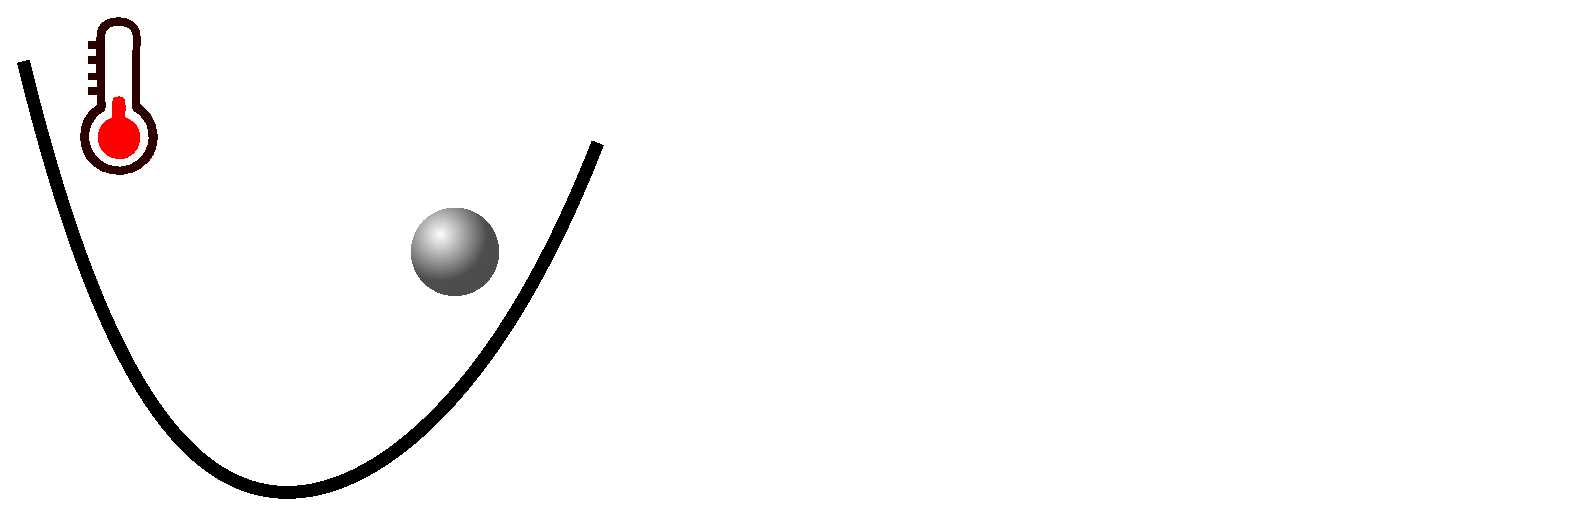
\includegraphics[width=0.7\textwidth]{iso-0.pdf}}%
             \onslide*<3>{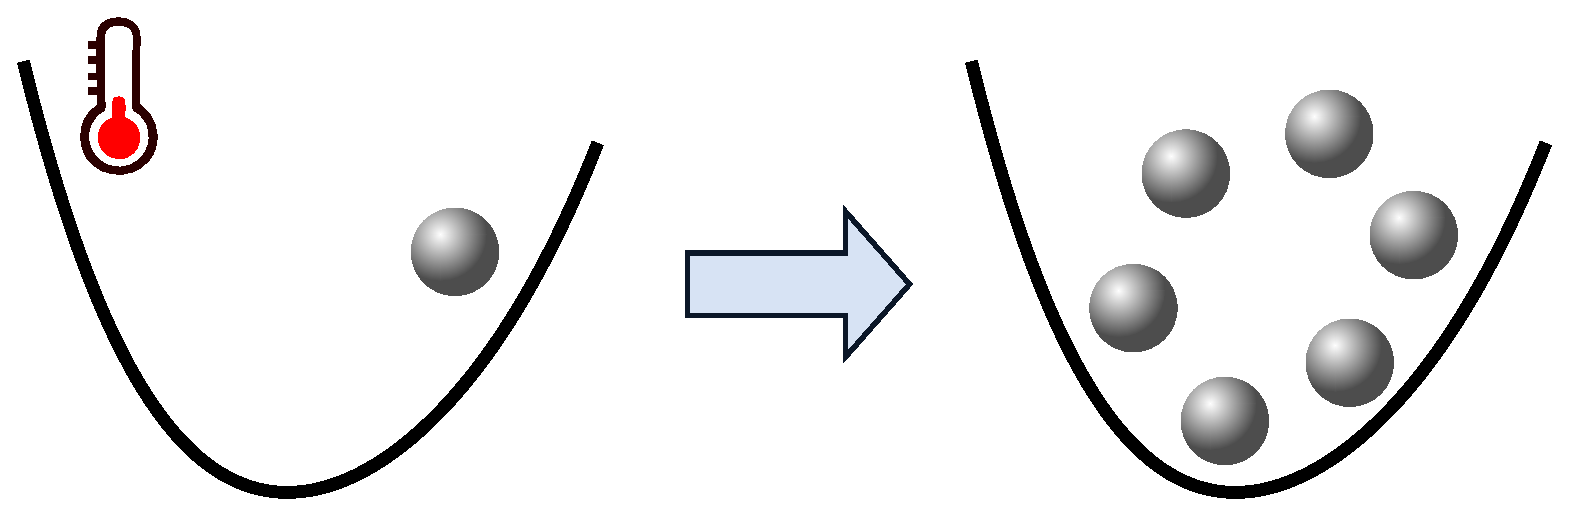
\includegraphics[width=0.7\textwidth]{iso-1.pdf}}%
             \onslide*<4>{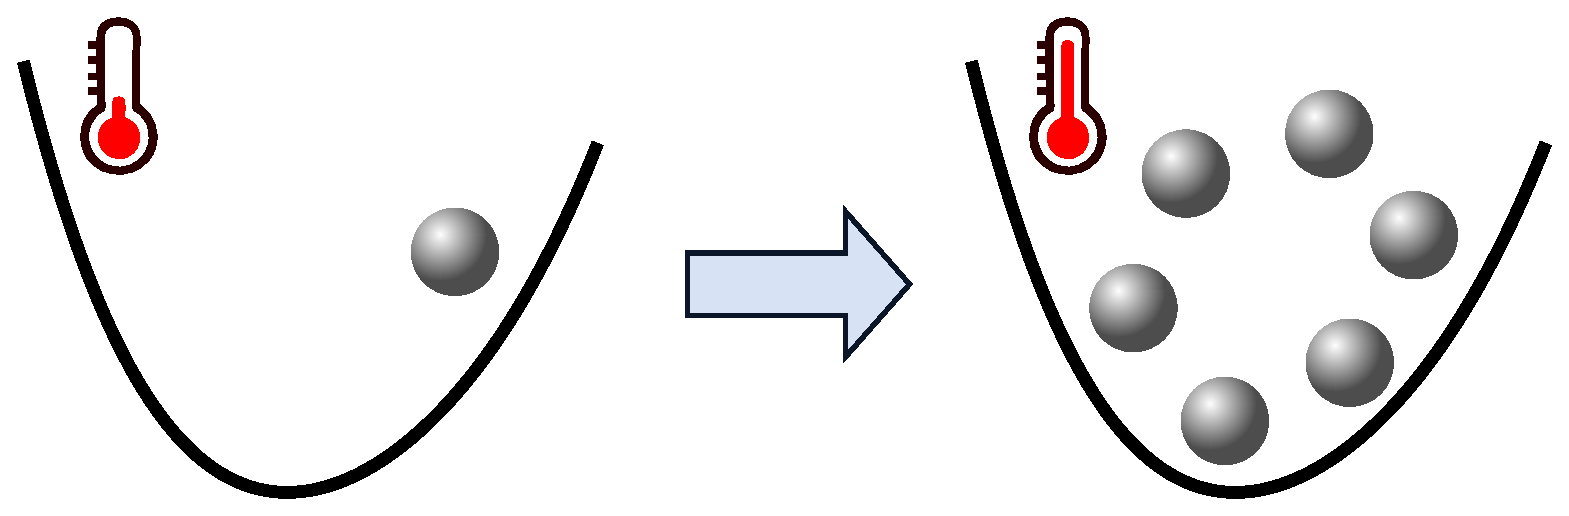
\includegraphics[width=0.7\textwidth]{iso-2.pdf}}%
            \onslide*<5->{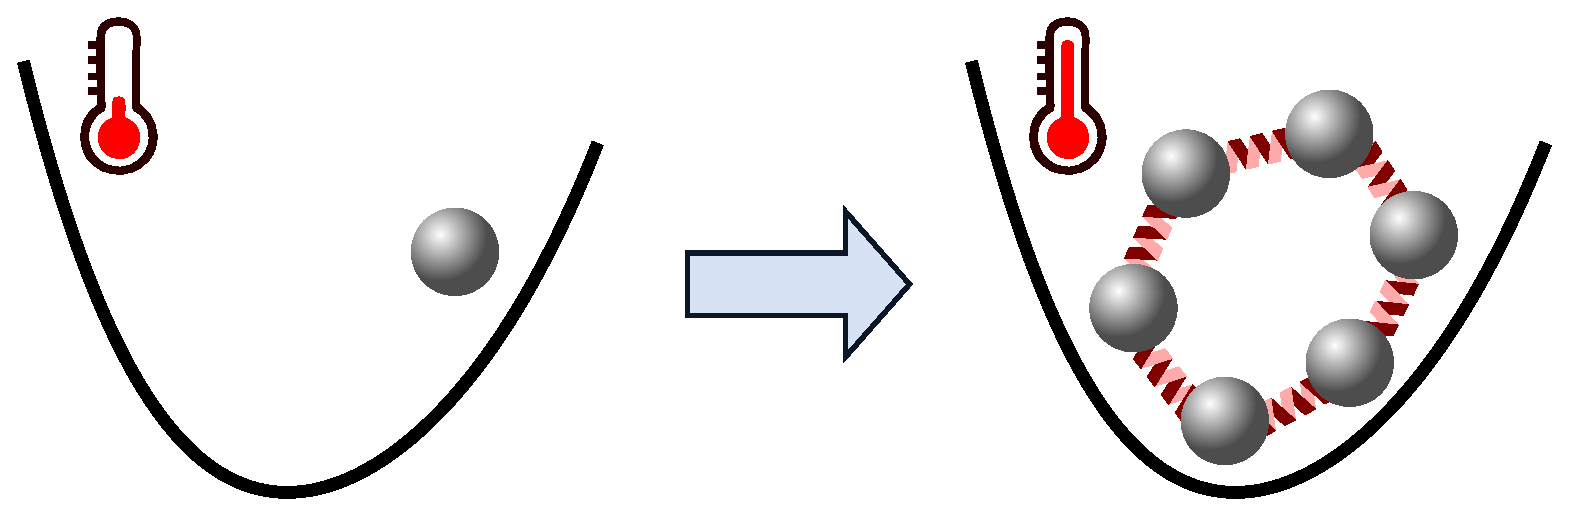
\includegraphics[width=0.7\textwidth]{iso-3.pdf}}
        \end{center}
    \end{overlayarea}
\end{frame}

\begin{frame}
    \frametitle{Thermal averages}

    % \[
    % \expval{A}_{\text{cl}} = \frac{1}{Z_{\text{cl}}} 
    %         \iint \dd{P} \dd{X} A(P, X) \, \eu[-\beta H(P,X)]
    % \]

    \[
    \expval{A}_{\text{qm}} = \frac{1}{Z} \Tr[\hat{A} \, \eu[-\beta \hat{H}]]
    \onslide*<2->{{}
    = \frac{1}{Z} \iint \dd[N]{P} \dd[N]{X} A_N(\boldsymbol{X}) \, \eu[\beta_N H_N(\boldsymbol{P}, \boldsymbol{X})] }
    \]

\bigskip

\begin{columns}[c]
    \begin{column}{0.45\textwidth}
        \onslide<3->{
        \begin{beamerboxesrounded}[lower=eqn,upper=eqn head,shadow=true]{\bfseries%
            Position estimators}
            \centering
            $ \displaystyle A_N(\boldsymbol{X}) = \frac{1}{N} \sum_{l=1}^{N} A(X_l) $
        \end{beamerboxesrounded}}
    \end{column}
    \begin{column}{0.45\textwidth}
        \begin{center}
        \onslide<4->{
        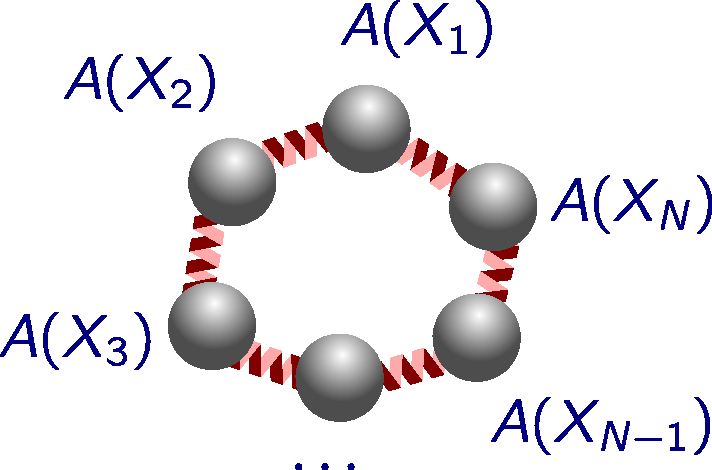
\includegraphics[width=0.8\textwidth]{estimator.pdf}}
        \end{center}
    \end{column}
\end{columns}

\end{frame}

\begin{frame}
    \frametitle{It's gone virial}

    \begin{textblock*}{\paperwidth}(85pt,85pt)
        \noindent
      \hspace*{2em}
      \onslide<2>{\rotatebox{30}{\color{red!70!black}{\bfseries\LARGE Trickery!}}}
    \end{textblock*}

    \begin{columns}[c]

        \begin{column}{0.60\textwidth}

            \alt{
            \begin{beamerboxesrounded}[lower=eqn,upper=eqn head,shadow=true]{
                \bfseries
                Primitive estimator}
                \centering
                \vspace*{1.75pt}
                $ \displaystyle
                K^{\text{p}}_N(\boldsymbol{X}) = \frac{N}{2 \beta}  
                    -\frac{1}{N} \sum_{l=1}^{N} \frac{M \omega_N^2 \qty(X_{l+1} - X_l)^2}{2} 
                $
            \end{beamerboxesrounded}
            }{
            \begin{beamerboxesrounded}[shadow=false]{\bfseries%
                    \vphantom{Primitive estimator}}
                    \centering
                    $ \displaystyle
                    \onslide*<1>{K_N(\boldsymbol{P}) \overset{?}{=} \frac{1}{N} \sum_{l=1}^{N} \frac{P_l^2}{2 M}}%
                    \onslide*<2>{\color{black!30}{K_N(\boldsymbol{P}) \overset{?}{=} \frac{1}{N} \sum_{l=1}^{N} \frac{P_l^2}{2 M}}}
                    % \onslide*<2>{K_N(\boldsymbol{P}, \boldsymbol{X}) = \frac{1}{N} \sum_{l=1}^{N} \frac{1}{2 M}
                    % \qty\Big( P_l + \iu M \omega_N (X_{l+1} - X_l) )^2}
                    $
            \end{beamerboxesrounded}
            }<3->

            \bigskip

            \onslide<4->{
            \begin{beamerboxesrounded}[lower=eqn,upper=eqn head,shadow=true]{
                \bfseries
                Centroid virial estimator}
                \centering
                \vspace*{1.75pt}
                $ \displaystyle
                K^{\text{cv}}_N(\boldsymbol{P}, \boldsymbol{X}) = \frac{1}{2 \beta}  
                    + \frac{1}{2 N} \sum_{l=1}^{N} (X_l - \bar{X}) \cdot \pdv{U(X_l)}{X_l}
                $
            \end{beamerboxesrounded}}
        \end{column}

        \begin{column}{0.35\textwidth}
            \vspace*{1em}
            \onslide<4->{
                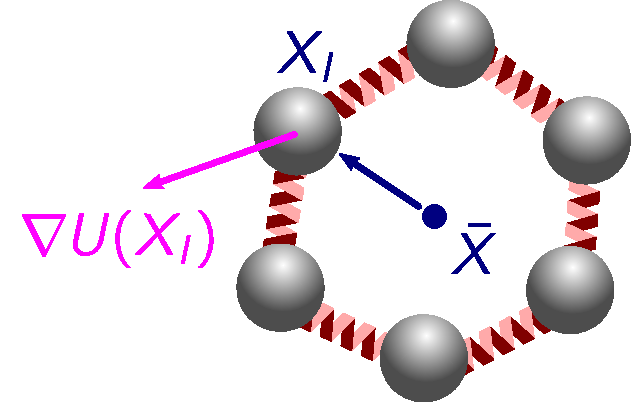
\includegraphics[width=\textwidth]{virial.pdf}}
            
        \end{column}

    \end{columns}
\end{frame}

\begin{frame}{The i-PI code}
\begin{center}
    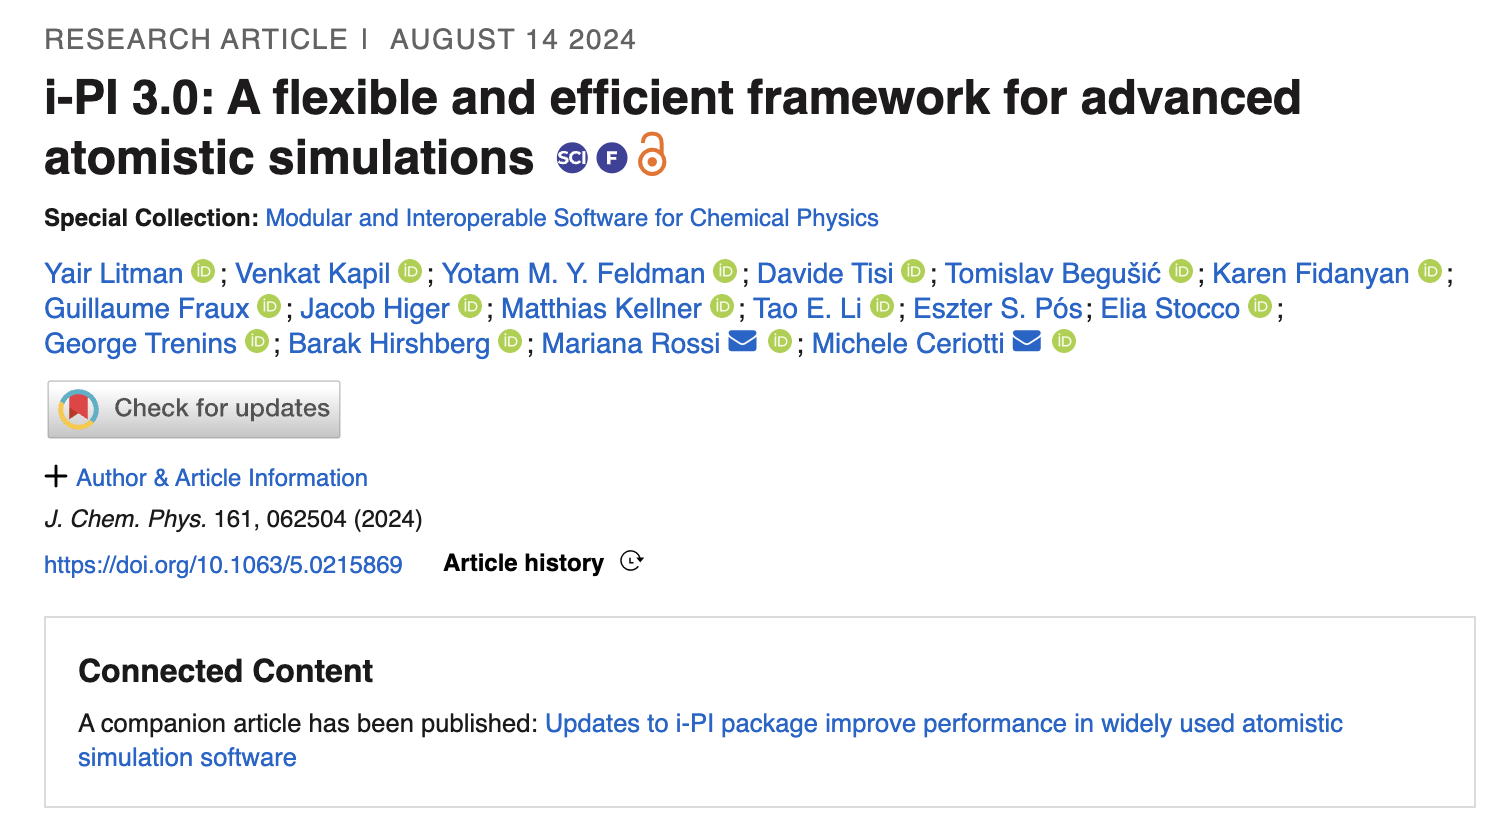
\includegraphics[width=0.9\textwidth]{graphics/ipi-paper.png}
\end{center}
\end{frame}

\begin{frame}{The i-PI code}
\vspace*{1em}
\begin{itemize}
    \setlength{\itemsep}{1em}
    \item The engine \emph{receives forces} and \emph{gives back positions}.
    \item Works for many kinds of ``motion'': dynamics, optimization, phonons, \ldots
    \item Electronic structure or ML potential acts as a simple driver (client).
\end{itemize}

\medskip

\begin{center}
    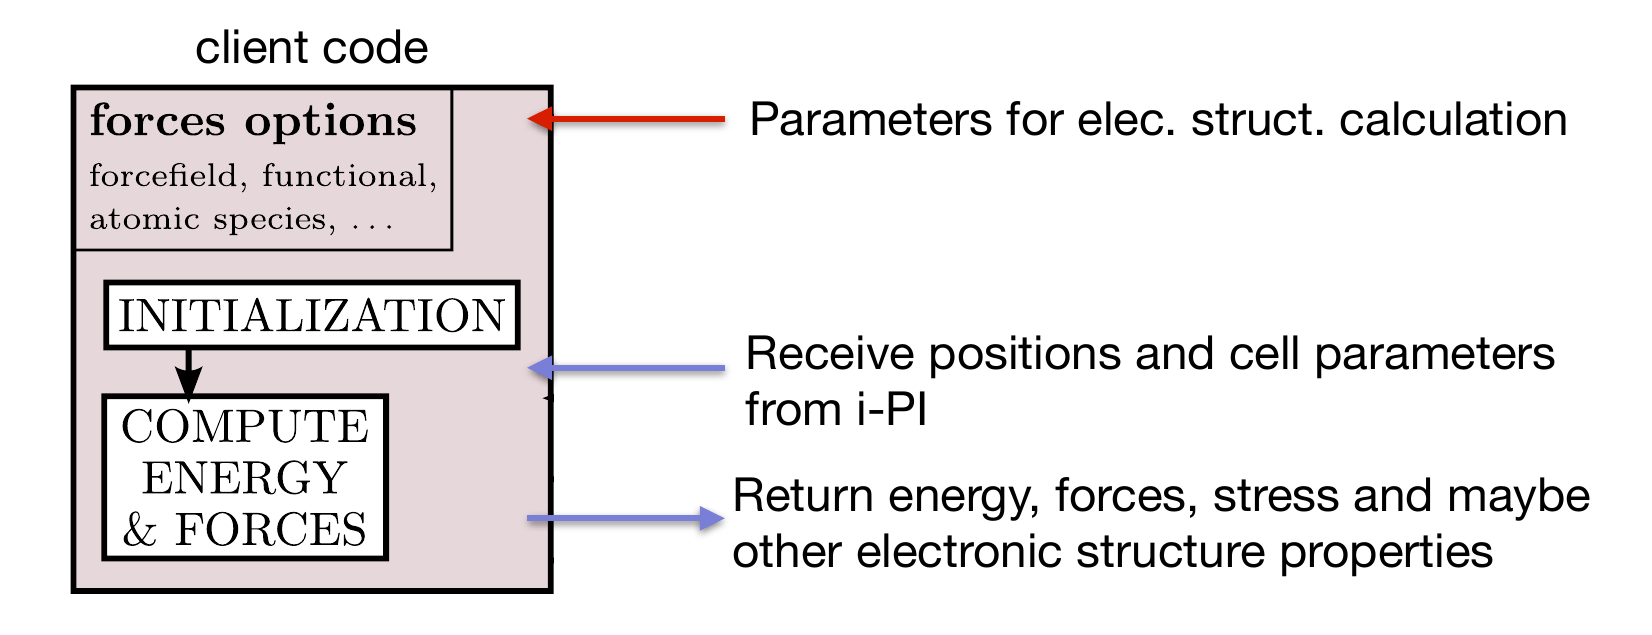
\includegraphics[width=0.75\textwidth]{graphics/ipi-driver.png}
\end{center}
\end{frame}

\begin{frame}{Communication via sockets}
    \begin{itemize}
        \setlength{\itemsep}{1em}
        \item i-PI communicates via internet (or UNIX) sockets
        \item Interfaced to: CP2K, DFTB+, \textbf{LAMMPS}, Quantum
ESPRESSO, \textbf{Siesta}, \textbf{FHI-aims}, Yaff, deMonNano, plumed, \textbf{ASE}, TBE, CASTEP, AMS, \ldots
    \end{itemize}

\bigskip

\begin{center}
    
\includegraphics[width=1.5in]{ipi-logo.pdf}
\end{center}

\begin{textblock*}{\paperwidth}(0pt,155pt)
      \hspace*{\fill}
      \parbox{2in}{
        Visit: \\
        \href{https://ipi-code.org/}{https://ipi-code.org/} \\
        \href{https://github.com/i-pi/i-pi}{https://github.com/i-pi/i-pi}
      }
\end{textblock*}
\end{frame}

\begin{frame}[plain]
\begin{center}
    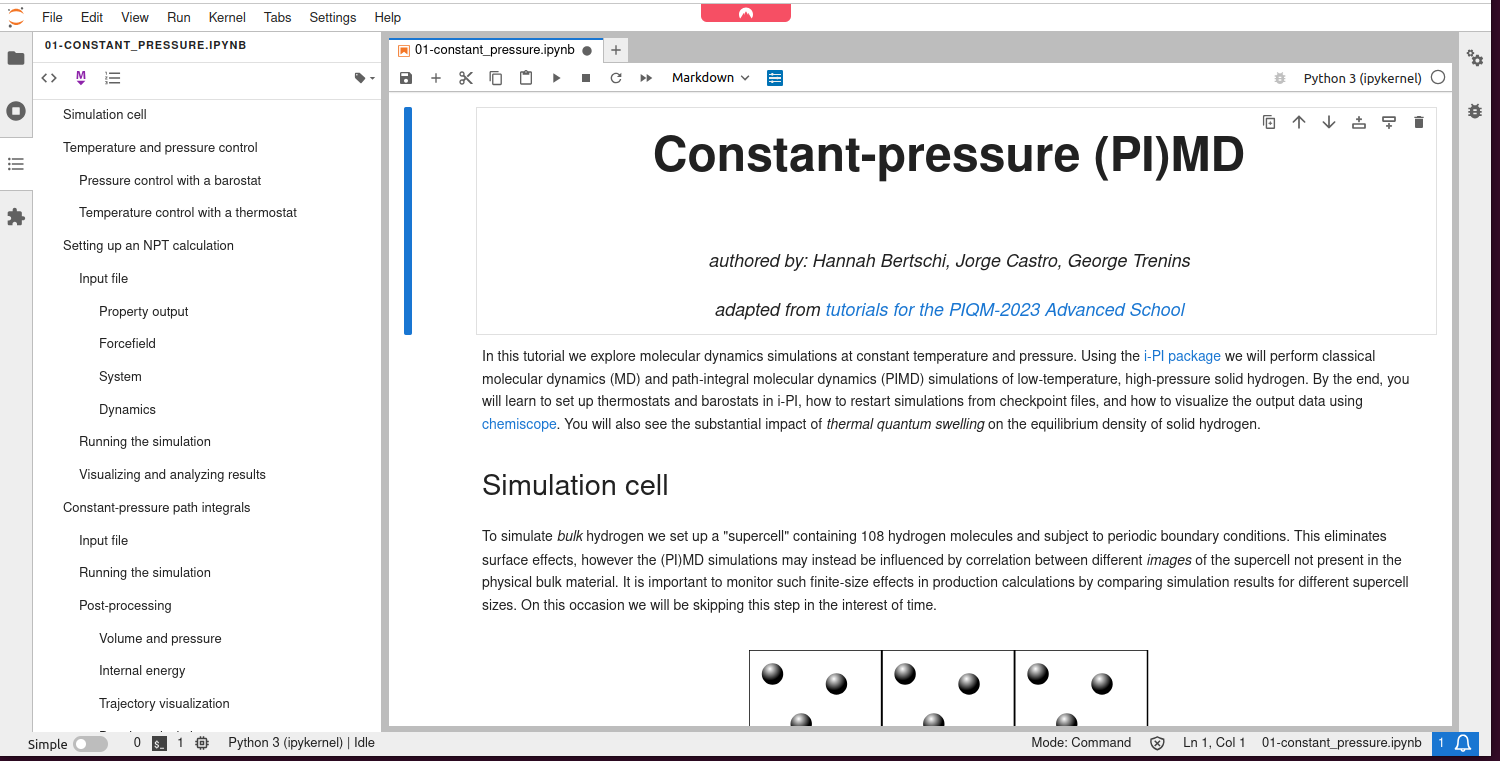
\includegraphics[width=\textwidth]{notebook.png}
\end{center}
\end{frame}

\begin{frame}
  \frametitle{``Kinetic'' matrix element}
  \hypertarget{deriv-slide}{}
  {\scriptsize\color{black}
  \begin{flalign*}
\shortintertext{\color{customblue}{\bfseries%
1. initial expression}}
    \mel{X_{l+1}}{ \eu[-\beta_N \hat{K}] }{X_l} & 
        =  \frac{1}{2 \pi \hbar} \int_{-\infty}^{\infty} \!\! 
        \dd{P'_l} \exp[-\frac{\beta_N P'^{2}_l }{2M} 
                    + \frac{\iu P'_l}{\hbar} (X_{l+1} - X_l)
                ] \vphantom{\exp[-\beta_N \frac{M \omega_N^2 (X_{l+1} - X_l)^{2}}{2}]} & \\
\shortintertext{\color{customblue}{\bfseries%
2. complete the square}}
       & = \frac{1}{2 \pi \hbar} \int_{-\infty}^{\infty} \!\! \dd{P'_l} 
                \exp[-\frac{\beta_N}{2M} 
                    \qty( P'_l - \frac{\iu M}{\beta_N\hbar} (X_{l+1} - X_l))^{\!2}] 
                \exp[-\beta_N \frac{M \omega_N^2 (X_{l+1} - X_l)^{2}}{2} 
                        \vphantom{ \qty( P'_l - \frac{\iu M}{\beta_N\hbar} (X_{l+1} - X_l))^{2}} ] & \\
\shortintertext{\color{customblue}{\bfseries%
3. change integration variable}}
        & = \frac{1}{2 \pi \hbar} \int_{-\infty-\iu \Delta_l}^{\infty- \iu \Delta_l} \dd{P_l} \exp[-\frac{\beta_N P_l^2}{2M}] \exp[-\beta_N \frac{M \omega_N^2 (X_{l+1} - X_l)^{2}}{2}]
        \qquad
         \color{commentgray} \left\{\mqty{
                \Delta_l = \mkern-2mu  \frac{M}{\beta_N\hbar} (X_{l+1} \mkern-2mu -  \mkern-2mu X_l) \\
                P_l =  P'_l - \iu \Delta_l }\right\} 
         & \\
\shortintertext{\color{customblue}{\bfseries%
4. deform integration contour}}
        & = \frac{1}{2 \pi \hbar} \int_{-\infty}^{\infty} \dd{P_l} \exp[-\frac{\beta_N P_l^2}{2M}] \exp[-\beta_N \frac{M \omega_N^2 (X_{l+1} - X_l)^{2}}{2}] &
  \end{flalign*}}


  \hspace*{\fill}\scalebox{1.2}{\hyperlink{ke-slide}{\beamerreturnbutton{Back to Main Slide}}}
\end{frame}

\end{document}
